\section{Kurvendiskussion}\label{sec:kurvendiskussion}

\begin{center}
    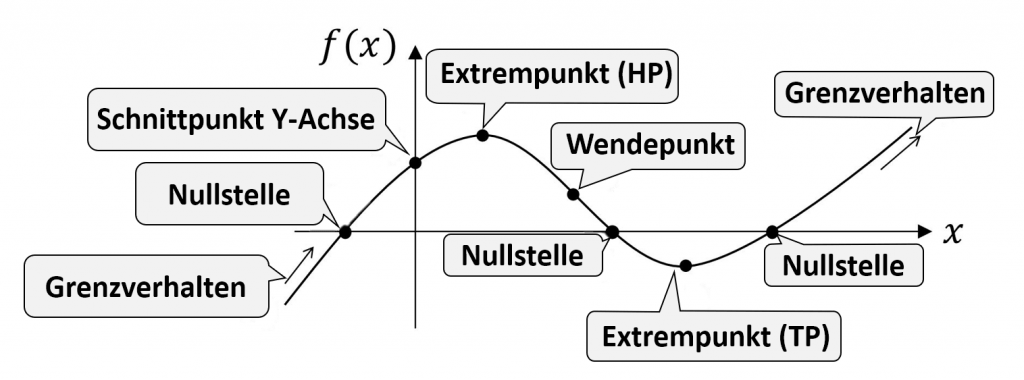
\includegraphics[scale=0.3]{kurvendiskussion}
\end{center}

\begin{definition}{Fragenkatalog für die Kurvendiskussion}
    \begin{enumerate}
        \item Definitionsbereich?
        \item Symmetrieeigenschaften (Gerade, ungerade, periode)?
        \item Schnittpunkte mit Achsen, Polstellen?
        \item Randpunkte bzw.\ Verhalten, wenn $x$ gegen die Grenzen des Definitionsbereichs strebt?
        \item Kandidaten für Extrema bestimmen und untersuchen
        \item Wendepunkte suchen
        \item Tabelle von Werten aufstellen (falls nötig)
    \end{enumerate}
\end{definition}